%%%%%%%%%%%%%%%%%%%%%%%%%%%%%%%%%%%%%%%%%%%%%%%%%%%%%%%%%%%%%%%%%%%%%%%%%%%%%%%%%%%%%%%%%%
%%
%% Description:		This is an example presentation using the beamerthemedhbw
%%
%%					The beamerthemedhbw is based on jacksbeamertheme
%%					(https://github.com/JacknJo/jacksbeamertheme)
%%
%% Author:			Hannes Bartle																				
%% 					DHBW Ravensburg Campus Friedrichshafen		
%%					September 2016	
%% 
%% The beamerthemedhbw is free software: you can redistribute it and/or modify
%% it under the terms of the GNU General Public License as published by
%% the Free Software Foundation, either version 3 of the License, or
%% (at your option) any later version.
%% 
%% The beamerthemedhbw is distributed in the hope that it will be useful,
%% but WITHOUT ANY WARRANTY; without even the implied warranty of
%% MERCHANTABILITY or FITNESS FOR A PARTICULAR PURPOSE.  See the
%% GNU General Public License for more details.
%% 
%% You should have received a copy of the GNU General Public License
%% along with the beamerthemedhbw.  If not, see <http://www.gnu.org/licenses/>.
%% 
%% 
%%%%%%%%%%%%%%%%%%%%%%%%%%%%%%%%%%%%%%%%%%%%%%%%%%%%%%%%%%%%%%%%%%%%%%%%%%%%%%%%%%%%%%%%%%


\documentclass[	12pt, 				
				t,					
				aspectratio=169,
				%handout-PLACEHOLDER
				]{beamer}

\usepackage{dhbwstyle}

\title{Generische Klassen\&Interfaces}


\begin{document}
	
	\begin{frame}[noframenumbering]
		\titlepage
	\end{frame}

	\begin{frame}{Inhalt}
		\tableofcontents
	\end{frame}
	
	\outlineFrame{Java-Klassenbibliothek}
	
	\begin{frame}{Java-Klassenbibliothek}{Kurzüberblick}
	\begin{itemize}
		\item Java bietet Vielzahl an "`fertigen"' Klassen
		\item Zusammengefasst in Packages
		\item Diese implementieren Standardfunktionalitäten wie z.B.
		\begin{itemize}
			\item Ein- und Ausgabefunktionalitäten
			\item Grafische Oberflächen
			\item Netzwerkkommunikation
			\item Datum- und Zeit, Internationalisierung
			\item Und viele mehr...
		\end{itemize}
	\end{itemize}
\end{frame}

\begin{frame}[allowframebreaks]{Wichtige Packages}{... der Klassenbibliothek}
Die wichtigsten Standardpackages im schnellen Überblick:
	\begin{itemize}
		\item \textit{java.lang}: Integriert die fundamentalen Klassen, die in der Regel immer zur Java Entwicklung benötigt werden wie zum Beispiel \texttt{String} \texttt{Object} oder auch die Wrapper Klassen der primitiven
		Datentypen (\texttt{Integer}, \texttt{Boolean}, \texttt{Double} usw.). \textbf{Muss nicht explizit importiert werden!}
		\item \textit{java.util}: Häufig benötigte Klassen, wie Listenstrukturen (\texttt{List}, \texttt{Stack}), Klassen zur Verarbeitung von Datum und Uhrzeit (\texttt{Calendar}) oder Zufallszahlengeneratoren (\texttt{Random})
		\item \textit{java.io}: Klassen zur Ein- und Ausgabe über Streams
		\item \textit{java.net}: Klasse zur Implementierung von Netzwerkkommunikation
		\item \textit{java.rmi}: Klassen zur Entwicklung verteilter Programme unter Nutzung von Remote Method Invocation
		\item \textit{java.awt}: Grundlegendes Package für die Entwicklung grafischer Oberflächen
		\item \textit{java.swing}: Erweiterte Komponente zur Entwicklung von grafischen Oberflächen. Baut auf \textit{java.awt} auf, bietet jedoch mehr Funktionalität
		\item \textit{javax.crypto} und \textit{java.security}: Klassen zur Umsetzung von sicherheitsrelevanten Aspekte (Zugriffsschutz, Rechteverwaltung etc.)
		\item \textit{java.sql}: Package zur Interaktion mit SQL Datenbanken
	\end{itemize}
\end{frame}

\begin{frame}{Arbeiten mit der Klassenbibliothek}
	\begin{itemize}
		\item Packages über \texttt{import} in Klasse einbinden
		\item Oracle bietet umfangreiche Dokumentation zu allen Klassen der Standard-API
		\item Schnellster Weg zur Doku:
		\begin{itemize}
			\item In den meisten IDEs sowieso integriert
			\item Sonst Google: "`Java 8/9/10 API \textit{PackageName}"'
		\end{itemize}
	\end{itemize}
\end{frame}

\begin{frame}{API-Dokumentation}{Links}
	\vfill
	\begin{block}{Java 8 API}
		\url{https://docs.oracle.com/javase/8/docs/api/index.html}
	\end{block}
	
	\begin{block}{Java 9 API}
		\url{https://docs.oracle.com/javase/9/docs/api/index.html}
	\end{block}
	
	\begin{block}{Java 10 API}
		\url{https://docs.oracle.com/javase/10/docs/api/index.html}
	\end{block}
	\vfill
\end{frame}
	
	\outlineFrame{Generische Klassen}
	
	\outlineSubframe{Motivation}
\begin{frame}{Generische Klassen}{Was ist das und Warum?}
	\begin{itemize}
		\item Ist eine Methode Klassen deutlich versatiler zu machen
		\begin{itemize}
			\item Und dadurch wiederverwenbar
			\item Bei geringerem Implementierungsaufwand
		\end{itemize}
		\item Bisher: Festlegen von Datentypen bei Design der Klasse
		\item Jetzt: Festlegen von Datentypen bei Verwendung der Klasse \visible<2->{(Zumindest für einige)}
		\item Funktioniert für:
		\begin{itemize}
			\item Member Variablen
			\item Funktionsparameter
			\item Rückgabewerte
		\end{itemize}
	\end{itemize}
\end{frame}

\begin{frame}{Generiche Klassen}{Beispiel: Benannte Werte}
	\begin{itemize}
		\item Angenommen man erhält folgende Anforderungen für eine Klasse
		\begin{itemize}
			\item Die Klasse soll einen Wert speichern
            \item Dieser soll vom Typ \texttt{Integer}, \texttt{String} oder \texttt{Boolean} sein
			\item Die Klasse soll einen Namen für diesen Wert als \texttt{String} speichern können
		\end{itemize}
		\item Mögliche Ansätze ohne generische Klassen:
		\begin{itemize}
			\item Implementierung einer Klasse \texttt{NamedValue}, die drei Member der entsprechenden Typen hat
			\item Implementierung einzelner Klassen \texttt{NamedInteger}, \texttt{NamedString} und \texttt{NamedBoolean}
		\end{itemize}
	\end{itemize}
\end{frame}

\begin{frame}[fragile]{Variante 1: One class for all!}{Implementierung}
\lstset{style=javacode}
\begin{lstlisting}
class NamedValue{
    private Integer intValue;
    private String stringValue;
    private Boolean boolValue;
    private String name;

    void set(Integer newInt);
    void set(String newString);
    void set(Boolean newBool);
    void setName(String newName);

    Integer getIntegerValue();
    String getStringValue();
    Boolean getBooleanValue();
    String getName();
}
\end{lstlisting}
\end{frame}

\begin{frame}{Variante 1: One class for all!}{Probleme}
    \begin{itemize}
        \item Es sollte \textbf{ein} Wert gespeichert werden
            \begin{itemize}
                \item Unsere Klasse speichert (theoretisch) bis zu drei verschiedene Werte
                \item \textit{Könnte} man abfangen
                \item Erhöht jedoch weiter den Implementierungsaufwand
            \end{itemize}
            \item Keine einheitliche Schnittstelle um Wert abzurufen
            \item Erhöhter Aufwand bei Erweiterung der Klasse
            \begin{itemize}
                \item Wert soll jetzt auch von Typ \texttt{Color} sein
                \item Hinzufügen neuer Member Variable \texttt{colorValue}
                \item Hinzufügen neuer set-/get-Methoden
            \end{itemize}
    \end{itemize}
\end{frame}

\begin{frame}[fragile]{Variante 2: Viel hilft viel!}{Implementierung \texttt{NamedInteger}}
\lstset{style=javacode}
\begin{lstlisting}
class NamedInteger{
    private Integer value;
    private String name;
    
    void set(Integer newValue);
    Integer get();
    
    void setName(String newName);
    String getName();
}
\end{lstlisting}
\end{frame}

\begin{frame}[fragile]{Variante 2: Viel hilft viel!}{Implementierung \texttt{NamedString}}
\lstset{style=javacode}
\begin{lstlisting}
class NamedString{
    private String value;
    private String name;
    
    void set(String newValue);
    String get();
    
    void setName(String newName);
    String getName();
}
\end{lstlisting}
\end{frame}

\begin{frame}[fragile]{Variante 2: Viel hilft viel!}{Implementierung \texttt{NamedBoolean}}
\lstset{style=javacode}
\begin{lstlisting}
class NamedString{
    private Boolean value;
    private String name;
    
    void set(Boolean newValue);
    Boolean get();
    
    void setName(String newName);
    String getName();
}
\end{lstlisting}
\end{frame}

\begin{frame}{Variante 2: Viel hilft viel!}{Probleme}
\begin{itemize}
    \item Löst einige Probleme der ersten Variante...
    \begin{itemize}
        \item Tatsächlich nur ein Wert gespeichert
        \item Einheitliche Schnittstelle
    \end{itemize}
    \item ...Aber eben nicht alle
    \item Copy-Paste-Code $\rightarrow$ Nach Möglichkeit zu vermeiden
    \item Problem bei Erweiterung bleibt ähnlich
    \begin{itemize}
        \item Würde hier neue Klasse erfordern
    \end{itemize}
\end{itemize}
\end{frame}


\outlineSubframe{Syntax\&Eigenschaften}

\begin{frame}{Generische Klassen}{Die Lösung des Problems!}
    \begin{itemize}
        \item Angabe von "`Platzhaltern"' bei Definition der Klasse
        \begin{itemize}
            \item Namen sind theoretisch beliebig wählbar
            \item ...Es gibt jedoch Naming conventions dazu
        \end{itemize}
        \item Diese repräsentieren den Datentypen
        \item Die Spezifizierung des Typs erfolgt erst bei Deklaration einer Variable vom Typ der Klasse
    \end{itemize}
\end{frame}

\begin{frame}[fragile]{Generische Klassen}{Syntax}
\lstset{style=javacode}
\begin{lstlisting}
class NamedValue<T>{
    private T value;
    private String name;
    
    void set(T newValue);
    T get();
    
    void setName(String newName);
    String getName();
}
//Verwendung:
NamedValue<Integer> namedInteger;
NamedValue<String> namedString;
NamedValue<Boolean> namedBoolean;
\end{lstlisting}
\end{frame}

\begin{frame}[fragile,allowframebreaks]{Eigenschaften von generischen Klassen}
\begin{itemize}
    \item Schnittstellen bleiben einheitlich (Im Rahmen des spezifizierten Typs)
    \item Kein Problem mit Anpassungen an neue Typen $\rightarrow$ Keine Änderung notwendig
    \item Definieren mehrerer generischer Typen möglich:
\end{itemize}%
\lstset{style=javacode}%
\begin{lstlisting}
class name<T1, T2, ..., Tn> {/*Klasseninhalt*/}
\end{lstlisting}
\framebreak
\begin{itemize}
\item Naming Conventions für Typen:
    \begin{itemize}
        \item In der Regel ein Buchstabe
        \item \texttt{T} - Type
        \item \texttt{E} - Element
        \item \texttt{N} - Number
        \item \texttt{K} - Key
        \item \texttt{V} - Value
    \end{itemize}
\end{itemize}
\end{frame}

\begin{frame}{Generische Klassen}{Begrenzen von Typen}
    \begin{itemize}
        \item Problem: Generics bieten nur begrenzte Funktionalität
        \begin{itemize}
            \item Garantiert sind nur Methoden die in \texttt{Object} implementiert sind
            \item \texttt{equals()}, \texttt{toString()}, \texttt{hashCode()}...
        \end{itemize}
        \item In manchen Fällen werden aber mehr Funktionalitäten benötigt
        \item Hierfür lassen sich Generics einschränken
        \begin{itemize}
            \item Nach benötigter Superklasse
            \item Nach benötigten Interfaces
        \end{itemize}
    \end{itemize}
\end{frame}

\begin{frame}[fragile]{Begrenzung von Typen}{Beispiel 1: Spezifizieren der Superklasse}
\lstset{style=javacode}
\begin{lstlisting}
class BoxedNumber<T extends Number>{
    private T number;
    
    void set(T newNumber);
    T get();
}
//Verwendung:
BoxedNumber<Interger> boxInt = new BoxedNumber<>();     //OK, Integer erbt von Number
BoxedNumber<Double> boxDbl = new BoxedNumber<>();       //OK, Double erbt von Number
BoxedNumber<String> error = new BoxedNumber<>();     //Compilerfehler, String ist keine Unterklasse von Number
\end{lstlisting}
\end{frame}

\begin{frame}[fragile]{Begrenzung von Typen}{Beispiel 2: Spezifizieren von Interfaces}
\lstset{style=javacode}
\begin{lstlisting}
class BoxedComparable<T extends Comparable<T>>{
    private T value;
    /* set()-/get()-Methoden */
    boolean isSmaller(T other){
        return value.compareTo(other)<0;
    }
}
//Verwendung:
BoxedComparable<Interger> boxInt;     //OK, Integer implementiert Comparable
BoxedComparable<String> boxString;    //OK
BoxedComparable<Color> error;         //Compilerfehler
\end{lstlisting}
\textbf{Achtung:} Auch für Interfaces wird in diesem Fall das keyword \texttt{extends} genutzt!
\end{frame}

\begin{frame}[fragile]{Begrenzung von Typen}{Beispiel 3: Spezifizieren von Superklasse\&Interfaces}
\lstset{style=javacode}
\begin{lstlisting}
class ComparableNumber<T extends Number&Comparable<T>>{
    private T value;
    
    void set(T newValue);
    T get();
    boolean isSmaller(T other){
        return value.compareTo(other)<0;
    }
}
//Verwendung:
ComparableNumber<Interger> compInt;      //OK
ComparableNumber<Double>  compDbl;        //OK
ComparableNumber<AtomicInteger> error;    //Compilerfehler
\end{lstlisting}
\end{frame}

\outlineSubframe{Generische Interfaces}

\begin{frame}{Generische Interfaces}{...Gibt es natürlich auch noch}
    \begin{itemize}
        \item Das ganze funktioniert analog mit Interfaces
        \item Klassen die das Interface implementieren müssen nicht generisch sein
        \item Spezifizierung des Typen erfolgt bei Implementierung
        \begin{itemize}
            \item Entweder direkte Angabe des Typen
            \item ...oder "`durchreichen"' von Typparametern der Klasse
        \end{itemize}
        \item Bekanntester Vertreter aus der Standardbibliothek: \texttt{Comparable<T>}
    \end{itemize}
\end{frame}

\begin{frame}[fragile]{Implementierung generischer Interfaces}{Beispiel 1: Direkte Angabe des Typen}
\lstset{style=javacode}
\begin{lstlisting}
class BoxedInt implements Comparable<Integer>{
    private Integer number;
    
    void set(Integer newNumber);
    Integer get();
    
    int compareTo(Integer i){
        return number.compareTo(i)
    }
}
\end{lstlisting}
\end{frame}

\begin{frame}[fragile]{Implementierung generischer Interfaces}{Beispiel 2: Durchreichen von Typparametern}
\lstset{style=javacode}
\begin{lstlisting}
class BoxedValue<T> implements Comparable<T>{
    private T value;
    
    void set(T newValue);
    T get();
    
    int compareTo(T o){
        if(number.hashCode()<i.hashCode()){
            return -1;
        } else if(number.hashCode()>i.hashCode()){
            return 1;
        } else{
            return 0;
        }
    }
}
\end{lstlisting}
\end{frame}

\outlineSubframe{Vererbung in Generischen Klassen}

\begin{frame}[fragile]{Vererbung}{Kurze Wiederholung}
\begin{minipage}{0.6\textwidth}
    \begin{itemize}
        \item Objekte von Subklassen können einem Objekt der Superklasse zugewiesen werden 
        \item So kann ein \texttt{Integer} beispielsweise einem \texttt{Object} zugewiesen werden
    \end{itemize}
    \lstset{style=javacode}
    \begin{onlyenv}<2->
    \begin{lstlisting}
Integer someInt = new Integer(42);
Object someObject = new Object();
someObject = someInt;   //OK
    \end{lstlisting}
    \end{onlyenv}
\end{minipage}%
\begin{minipage}{0.35\textwidth}
\centering
    \begin{figure}
        \centering
        \visible<3->{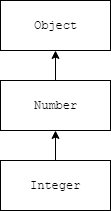
\includegraphics[width=2.5cm]{graph/int2obj}}
    \end{figure}
\end{minipage}
\end{frame}

\begin{frame}[fragile]{Vererbung}{In generischen Klassen}
    \begin{itemize}
        \item Gleiches gilt natürlich auch für den generischen Typ selbst
        \item<2-> Zum Beispiel bei Funktionsaufrufen können auch Objekte der Subklasse übergeben werden:
    \end{itemize}
    \lstset{style=javacode}
    \begin{onlyenv}<3->
    \begin{lstlisting}
class BoxValue<T>{
    private T val;
    
    void set(T t);
    T get();
}
//Erlaubte Verwendung:
BoxValue<Number> boxNum = new BoxValue();
boxNum.set(new Double(2.34));   //OK
boxNum.set(new Integer(7));     //OK
    \end{lstlisting}
    \end{onlyenv}
\end{frame}

\begin{frame}[fragile]{Vererbung}{Von generischen Klassen}
\lstset{style=javacode}
\begin{lstlisting}
void someMethod(BoxValue<Number> box){/* ... */}
\end{lstlisting}
\begin{itemize}
    \item<2-> Welche Typen werden akzeptiert?
    \begin{itemize}
        \item<3-> \texttt{BoxValue<Number>}
        \item<4-> \texttt{BoxValue<Integer>}?
        \item<5-> \texttt{BoxValue<Double>}?
    \end{itemize}
    \item<6-> \textbf{NUR} \texttt{BoxValue<Number>} wird als Typ akzeptiert
    \item<7-> \texttt{Integer} erbt zwar von \texttt{Number}...
    \begin{itemize}
        \item<8-> ...Aber \texttt{BoxValue<Number>} und \texttt{BoxValue<Integer>} stehen in keiner Beziehung zueinander!
    \end{itemize}
\end{itemize}
\end{frame}

\begin{frame}{Vererbung}{Von generischen Klassen}
    \begin{figure}
        \centering
        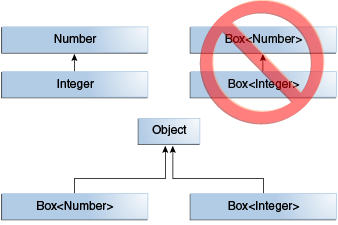
\includegraphics[height=4.5cm]{graph/generics-subtypeRelationship.png}
        \caption*{Quelle: \url{https://docs.oracle.com/javase/tutorial/java/generics/inheritance.html}}
    \end{figure}
\end{frame}

    
    \outlineSubframe{Wildcards}
    \outlineSubframe{Einschränkungen}
    %TODO:
    %Generic Interfaces
    %Wildcards

    \section*{Kontakt}
	\begin{frame}{Kontakt}{}
	\begin{itemize}
		\item E-Mail: \href{mailto:lukas.abelt@airbus.com}{lukas.abelt@airbus.com}
		\item GitHub: \url{https://www.github.com/LuAbelt}
		\item GitLab: \url{https://www.gitlab.com/LuAbelt}
		\item Telefon(Firma): 07545 - 8 8895
		\item Telegram: LuAbelt
	\end{itemize}
\end{frame}
	

\end{document}